\let\negmedspace\undefined
\let\negthickspace\undefined
\documentclass[journal]{IEEEtran}
\usepackage[a5paper, margin=10mm, onecolumn]{geometry}
%\usepackage{lmodern} % Ensure lmodern is loaded for pdflatex
\usepackage{tfrupee} % Include tfrupee package

\setlength{\headheight}{1cm} % Set the height of the header box
\setlength{\headsep}{0mm}     % Set the distance between the header box and the top of the text

\usepackage{gvv-book}
\usepackage{gvv}
\usepackage{cite}
\usepackage{amsmath,amssymb,amsfonts,amsthm}
\usepackage{algorithmic}
\usepackage{graphicx}
\usepackage{textcomp}
\usepackage{xcolor}
\usepackage{txfonts}
\usepackage{listings}
\usepackage{enumitem}
\usepackage{mathtools}
\usepackage{gensymb}
\usepackage{comment}
\usepackage[breaklinks=true]{hyperref}
\usepackage{tkz-euclide} 
\usepackage{listings}
% \usepackage{gvv}                                        
\def\inputGnumericTable{}                                 
\usepackage[latin1]{inputenc}                                
\usepackage{color}                                            
\usepackage{array}                                            
\usepackage{longtable}                                       
\usepackage{calc}                                             
\usepackage{multirow}                                         
\usepackage{hhline}                                           
\usepackage{ifthen}                                           
\usepackage{lscape}
\begin{document}

\bibliographystyle{IEEEtran}
\vspace{3cm}

\title{1-1.9-24}
\author{AI24BTECH11015 - Harshvardhan Patidar}
 \maketitle
% \newpage
% \bigskip
{\let\newpage\relax\maketitle}

\renewcommand{\thefigure}{\theenumi}
\renewcommand{\thetable}{\theenumi}
\setlength{\intextsep}{10pt} % Space between text and floats


\numberwithin{equation}{enumi}
\numberwithin{figure}{enumi}
\renewcommand{\thetable}{\theenumi}


	Question:\\
		The $x$-coordinate of a point $\vec{P}$ twice its $y$-coordinate. If $\vec{P}$ is equidistant from the points $\vec{Q} \myvec{2&-5}$ and $\vec{R} \myvec{-3&6}$, find the coordinates of $\vec{P}$.\\ \\


	\solution\\
		\begin{table}[h!]    
  			\centering
  			\begin{tabular}[12pt]{ |c| c|}
    \hline
    \textbf{Variable} & \textbf{Description}\\
    \hline
	$\vec{m}$ & Unit Vector\\
    \hline
	$\alpha$ & Angle of the unit vector with $x$-axis\\
    \hline
	$\beta$ & Angle of the unit vector with $y$-axis\\
    \hline	
    \end{tabular}

  			\caption{Variables Used}
  			\label{tab1-1.9-24}
		\end{table}\\

		
		Now, since $\vec{P}$ is equidistant from $\vec{Q}$ and $\vec{R}$,
			\begin{align}
				\norm{P - Q}  &=  \norm{ P - R }\\
				\sqrt{\brak{P-Q}^T\brak{P-Q}}&=\sqrt{\brak{P-R}^T\brak{P-R}} \label{eqn}
			\end{align}

			$$ \brak{P-Q} = \myvec{2a-2\\a+5}, \brak{P-R} = \myvec{2a+3\\a-6}$$

			Putting values into equation \eqref{eqn} and squaring,
			\begin{align}	
				(2a-2)^2 + (a+5)^2 &= (2a+3)^2 + (a-6)^2\\
				a &= 8
			\end{align}

			So, 
			\begin{align}
				\vec{P} = \myvec{16\\8}
			\end{align}

			               
	\begin{figure}[H]
		\centering
		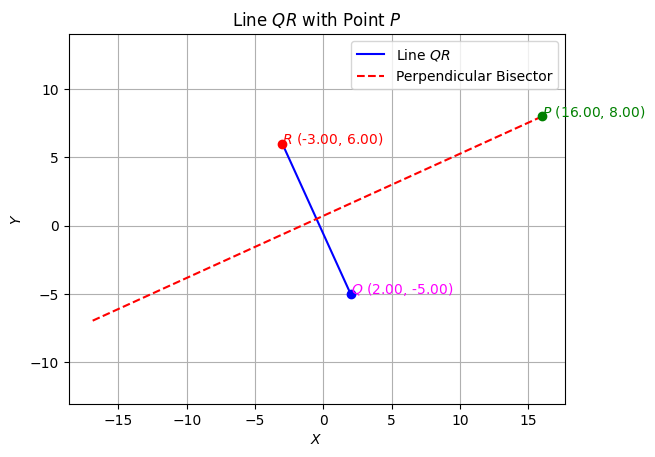
\includegraphics[width=\textwidth]{plots/plot.png}
	\end{figure}
		
  
\end{document}
				



				%Let $y$-coordinate of $\vec{P}$ be $a$.\\
				%Then, 
				%	\begin{align*}
				%		\vec{P} = \myvec{2a\\a}
				%	\end{align*}


				%\lVert \vec{P} - \vec{Q} \rVert ^ 2  &=  \lVert \vec{P} - \vec{R} \rVert ^ 2\\
				%\vec{P}^2 + \vec{Q}^2 - 2 \vec{P}\vec{Q}^{\top} &= \vec{P}^2 + \vec{R}^2 - 2\vec{P}\vec{R}^{\top}\\
				%2\vec{P} \brak{\vec{R}^{\top} - \vec{Q}^{\top}} &= \vec{R}^2 - \vec{Q}^2\\
				%\myvec{2a\\a}\myvec{-5&11} &= 8 \\
				%a&=8



